\documentclass[11pt,xcolor=table]{beamer}

\usetheme[progressbar=frametitle]{metropolis}
\usepackage{appendixnumberbeamer}
\usepackage{pgfpages}
%\setbeameroption{show notes on second screen}
  \setbeamertemplate{enumerate items}[square]
\usepackage{multirow}

\usepackage{graphicx}

\usepackage{xcolor}

\newcommand{\link}[3][mLightBrown]{\href{#2}{\color{#1}{#3}}}%


\newcommand{\questionslide}[0]{
{\setbeamercolor{palette primary}{fg=black, bg=yellow}
\begin{frame}[standout]
    \raggedright
  Any questions? \\ \vspace{1cm}
  \raggedleft
  \dots{ } Remember -- Every question is useful!
\end{frame}
}}

\newcommand{\task}[1]{
   \begin{alertblock}
   {\centering \vspace{-1.5ex} \\ #1  \\ \vspace{-1.5ex} }
   \end{alertblock}
   }

\setbeamercolor{block title alerted}{%
    use={block title, alerted text},
    bg=yellow,
    fg=black
}

\definecolor{peppermint}{RGB}{75, 161, 115}
%\definecolor{peppermint}{RGB}{75, 161, 115}


\setbeamercolor{alerted text}{fg=peppermint , bg= black}

\usepackage{booktabs}
\usepackage[scale=2]{ccicons}

\usepackage{pgfplots}
\usepgfplotslibrary{dateplot}

\makeatletter 
\def\beamer@framenotesbegin{% at beginning of slide
    \usebeamercolor[fg]{normal text}
    \gdef\beamer@noteitems{}% 
    \gdef\beamer@notes{}% 
}
\makeatother


\usepackage{xspace}
\newcommand{\themename}{\textbf{\textsc{metropolis}}\xspace}

\title{Introduction to Instrumental Variables
}
\subtitle{Econ 140, Section 7}
% \date{\today}
\date{}
\author{Jonathan Old}

% \titlegraphic{\hfill\includegraphics[height=1.5cm]{logo.pdf}}

\begin{document}

\maketitle

\begin{frame}{Roadmap}
  \setbeamertemplate{section in toc}[sections numbered]
  \tableofcontents%[hideallsubsections]
\end{frame}




\questionslide



\section{(Group) data projects}



\begin{frame}{Your time for questions}
I prepared a document that can help you find data if you are lost. See it on  \link{https://bcourses.berkeley.edu/courses/1538138/files/folder/Sections/101\%20102\%20-\%20Jonathan}{bCourses}.

The first deadline is this Sunday night.

Group work encouraged!

\end{frame}




\section{Introduction to Instrumental Variables}

\begin{frame}{Recap: Omitted Variable Bias}
    \begin{figure}
        \centering
        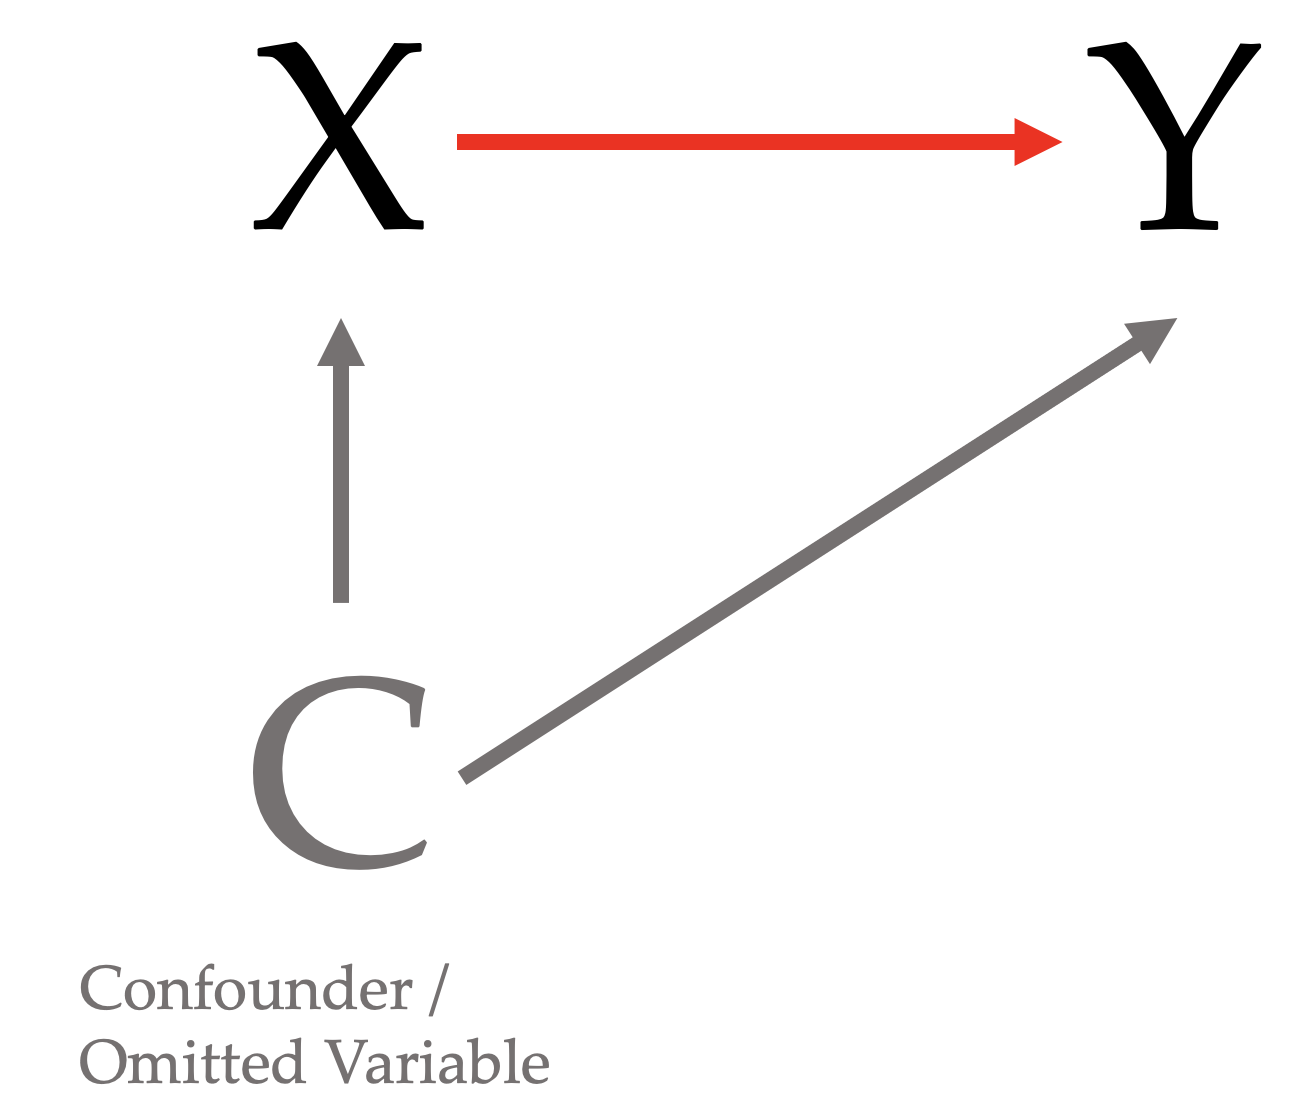
\includegraphics[width=0.5\textwidth]{DAGs/ovb.png}
       % \caption{IV setup}
        \label{fig:ovb}
    \end{figure}
\end{frame}



\begin{frame}{Instrumental variables: The setup}
    \begin{figure}
        \centering
        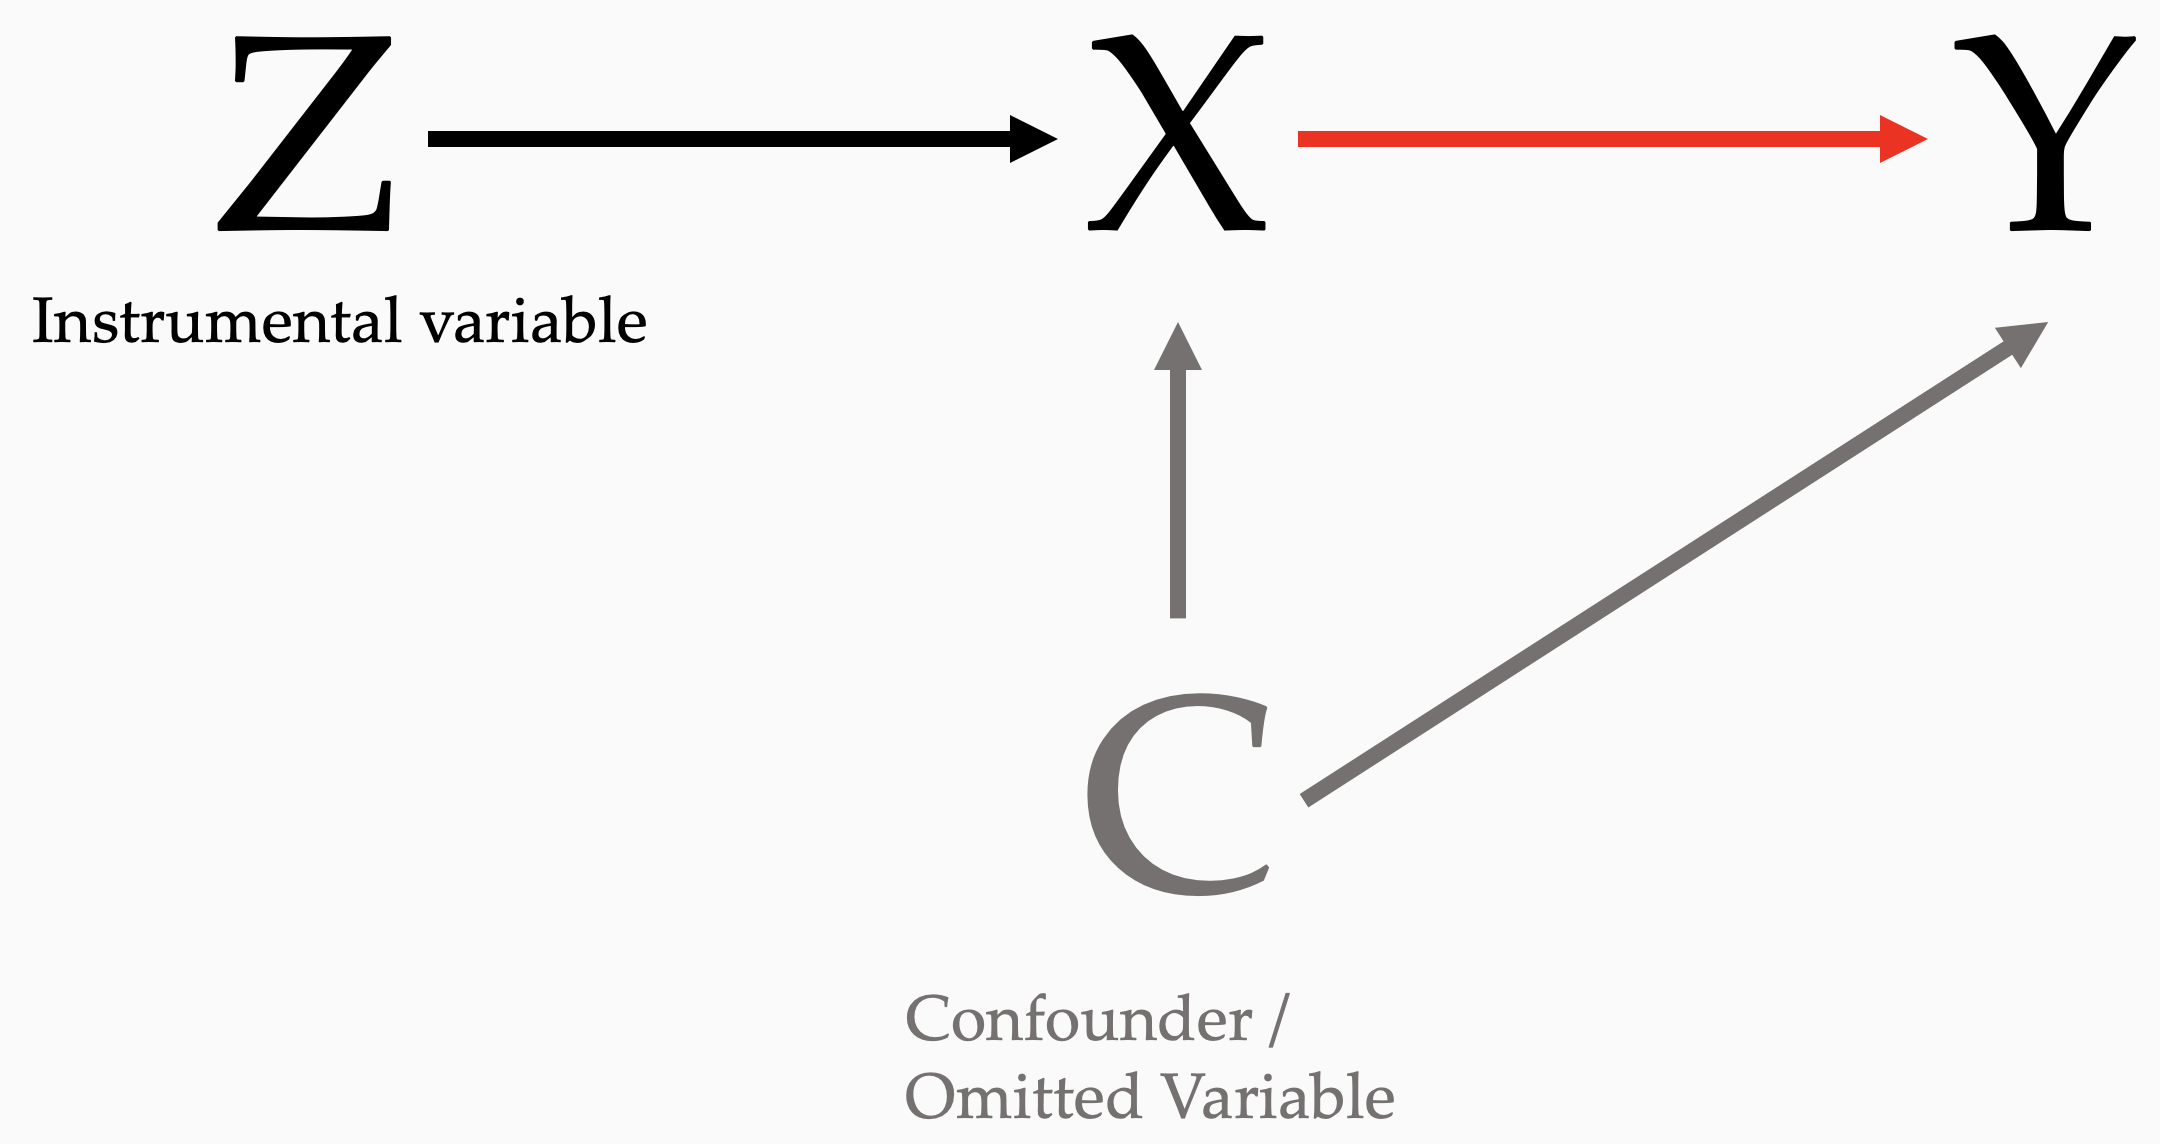
\includegraphics[width=0.8\textwidth]{DAGs/iv_simple.png}
       % \caption{IV setup}
        \label{fig:iv}
    \end{figure}
\end{frame}



\begin{frame}{Recap: IV "rescales" the effect}
    \begin{figure}
        \centering
        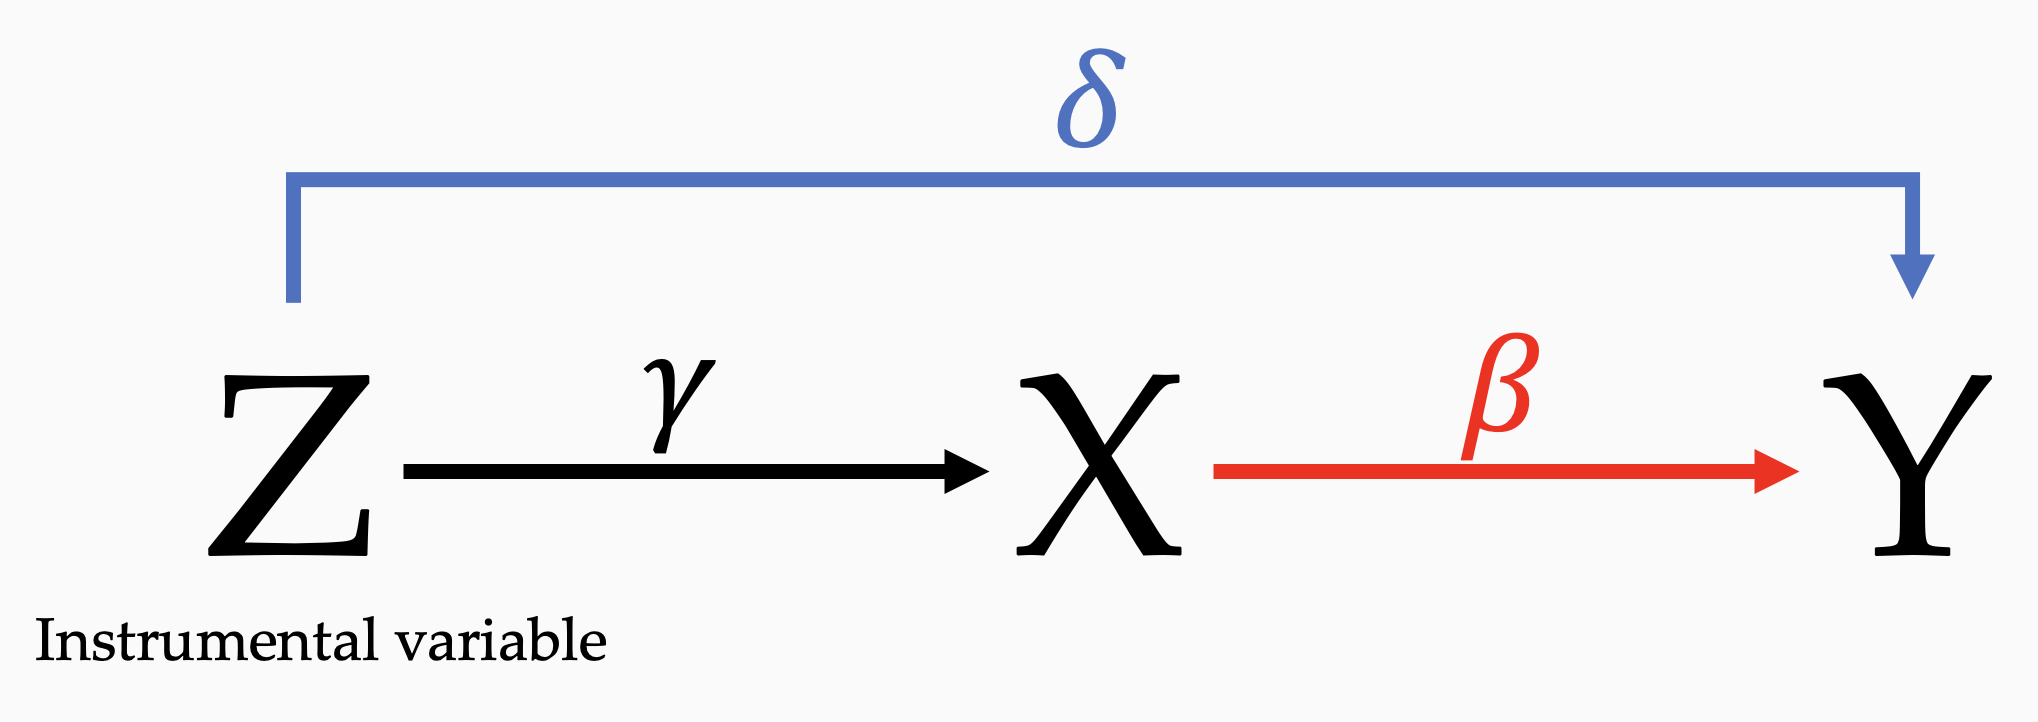
\includegraphics[width=0.75\textwidth]{DAGs/iv_calc.png}
       % \caption{We can calculate $\beta$ as $\delta / \gamma $.}
        \label{fig:iv2}
    \end{figure}
    
    A simple example: 
    \begin{itemize}
    \item We want to know the effect of chocolate ($X$) on happiness ($Y$), using a randomized voucher as instrument ($Z$). 
    \item We find: people with voucher were 3 points more happy ($\delta = 3$), and ate  0.5 more chocolates ($\gamma=0.5$).
    \item Then, the effect of eating one more chocolate is: \pause  $\beta = \delta / \gamma = 3/0.5= 6$.
    \end{itemize}
\end{frame}



\begin{frame}{Calculating the IV coefficient}
    
What is the effect of \textbf{eating chocolate} (D) on happiness (Y).
\begin{itemize}
    \item Why not estimate: $Y_i = \alpha + \beta D_i + \varepsilon_i$?
\end{itemize}
\textbf{Randomly} give voucher to buy chocolate at $90 \%$ discount (Z).

\begin{itemize}
    \item Why not estimate: $Y_i = \alpha + \beta Z_i + \varepsilon_i$?
\end{itemize}
\textbf{Let us set up some regressions}:
\begin{align*}
\text{Regression of interest: }  Y_i&=\alpha+\beta  D_i +  e_i \\
\text{First stage: }  D_i&=\alpha_1+\gamma  Z_i + u_i \\
\text{Reduced Form: }  Y_i&=\alpha_2+\delta  Z_i + v_i \\
\text{Plug in regression of interest: }  Y_i &= \alpha + \beta (\alpha_1+\gamma \cdot Z_i + u_i) + e_i   \\ 
\text{Get back reduced form: \qquad }& = \underbrace{(\alpha + \beta \alpha_1)}_{\alpha_2} + \underbrace{(\beta \gamma)}_{\delta} Z_i + \underbrace{(\beta u_i + e_i)}_{v_i}  \\
 \text{So we see that} \qquad    \delta = \beta \gamma &\Leftrightarrow \beta = \delta / \gamma
\end{align*}





\end{frame}



\begin{frame}{Interpretation of the IV coefficient}
\begin{itemize}
\item How do we interpret $\gamma$ ? \pause The average difference in chocolate consumption between those who got a voucher and those who didn't \pause 
\item How do we interpret $\delta$ ? \pause The average difference in happiness between those who got a voucher and those who didn't \pause 
\end{itemize}
$$
\beta=\frac{\gamma}{\delta}=\frac{E\left[Y_i \mid Z_i=1\right]-E\left[Y_i \mid Z_i=0\right]}{E\left[D_i \mid Z_i=1\right]-E\left[D_i \mid Z_i=0\right]}
$$


\end{frame}



\begin{frame}{IV gives us the treatment effect for the compliers}

\begin{figure}
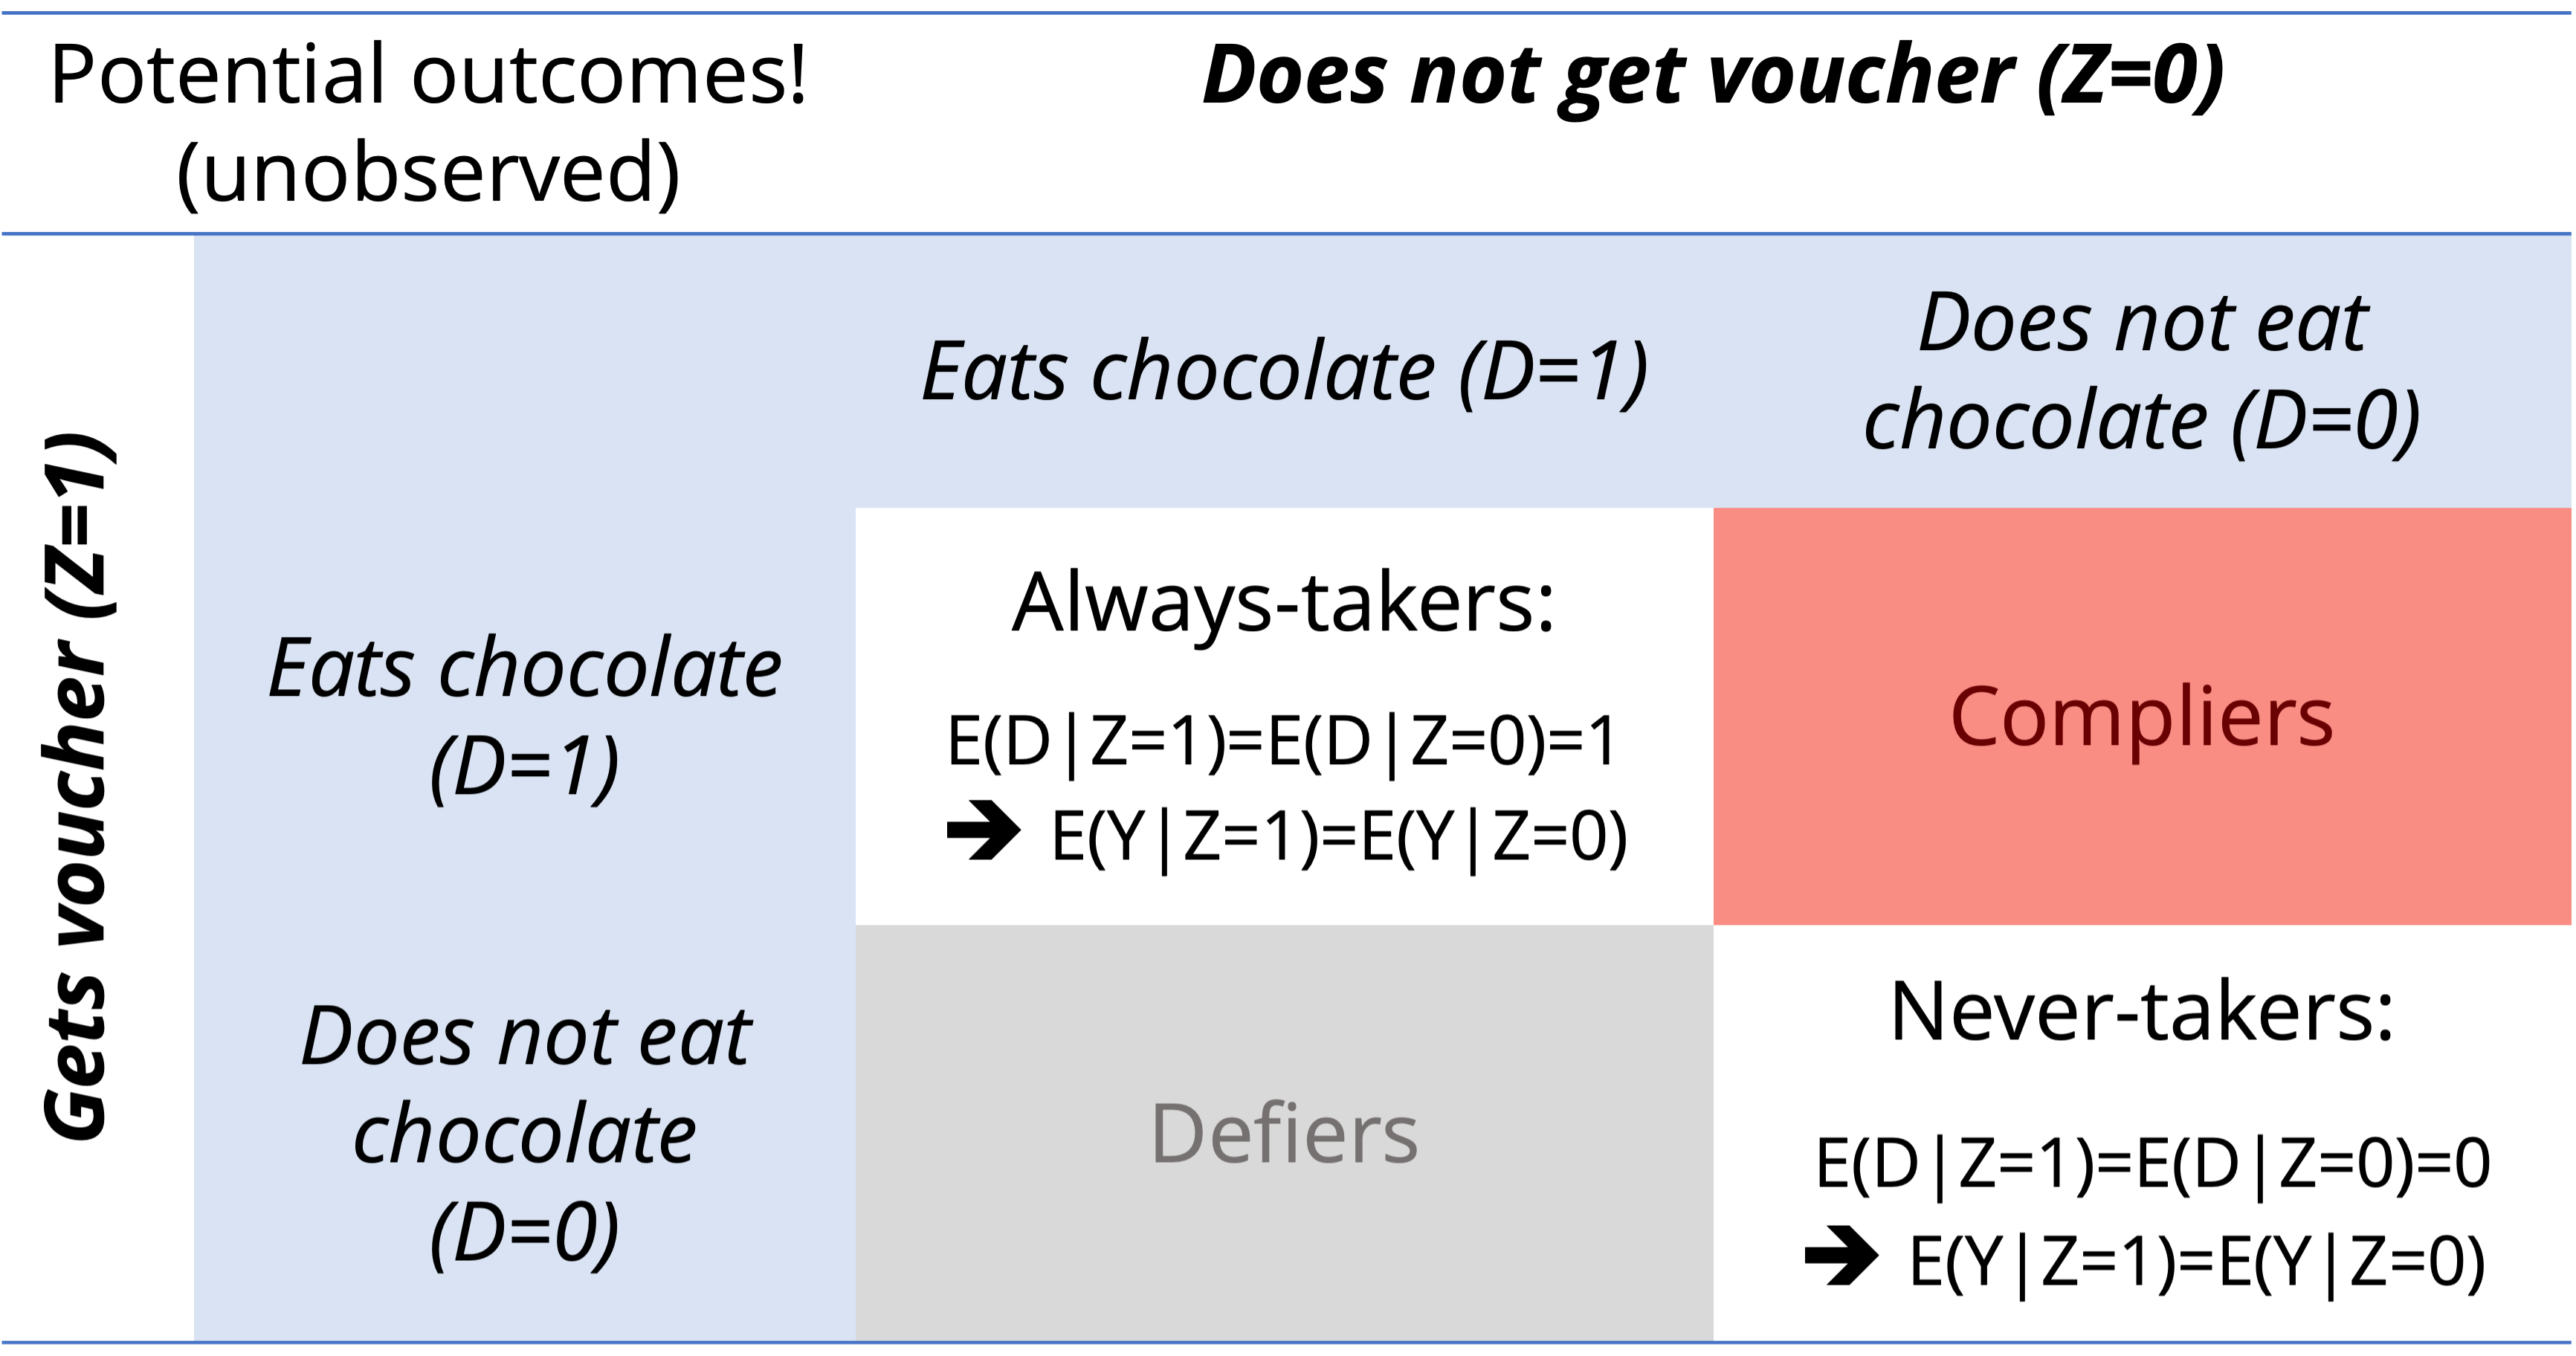
\includegraphics[width=\textwidth]{figures/iv_table.png}
\end{figure}

\end{frame}


\section{IV Conditions}

\begin{frame}{Does IV always work?}

\begin{itemize}
    \item No! It only works if we have a valid instrument
    \item For this, we need three conditions:
\end{itemize}

1. Relevance: $Z$ must truly affect $X$
\begin{figure}
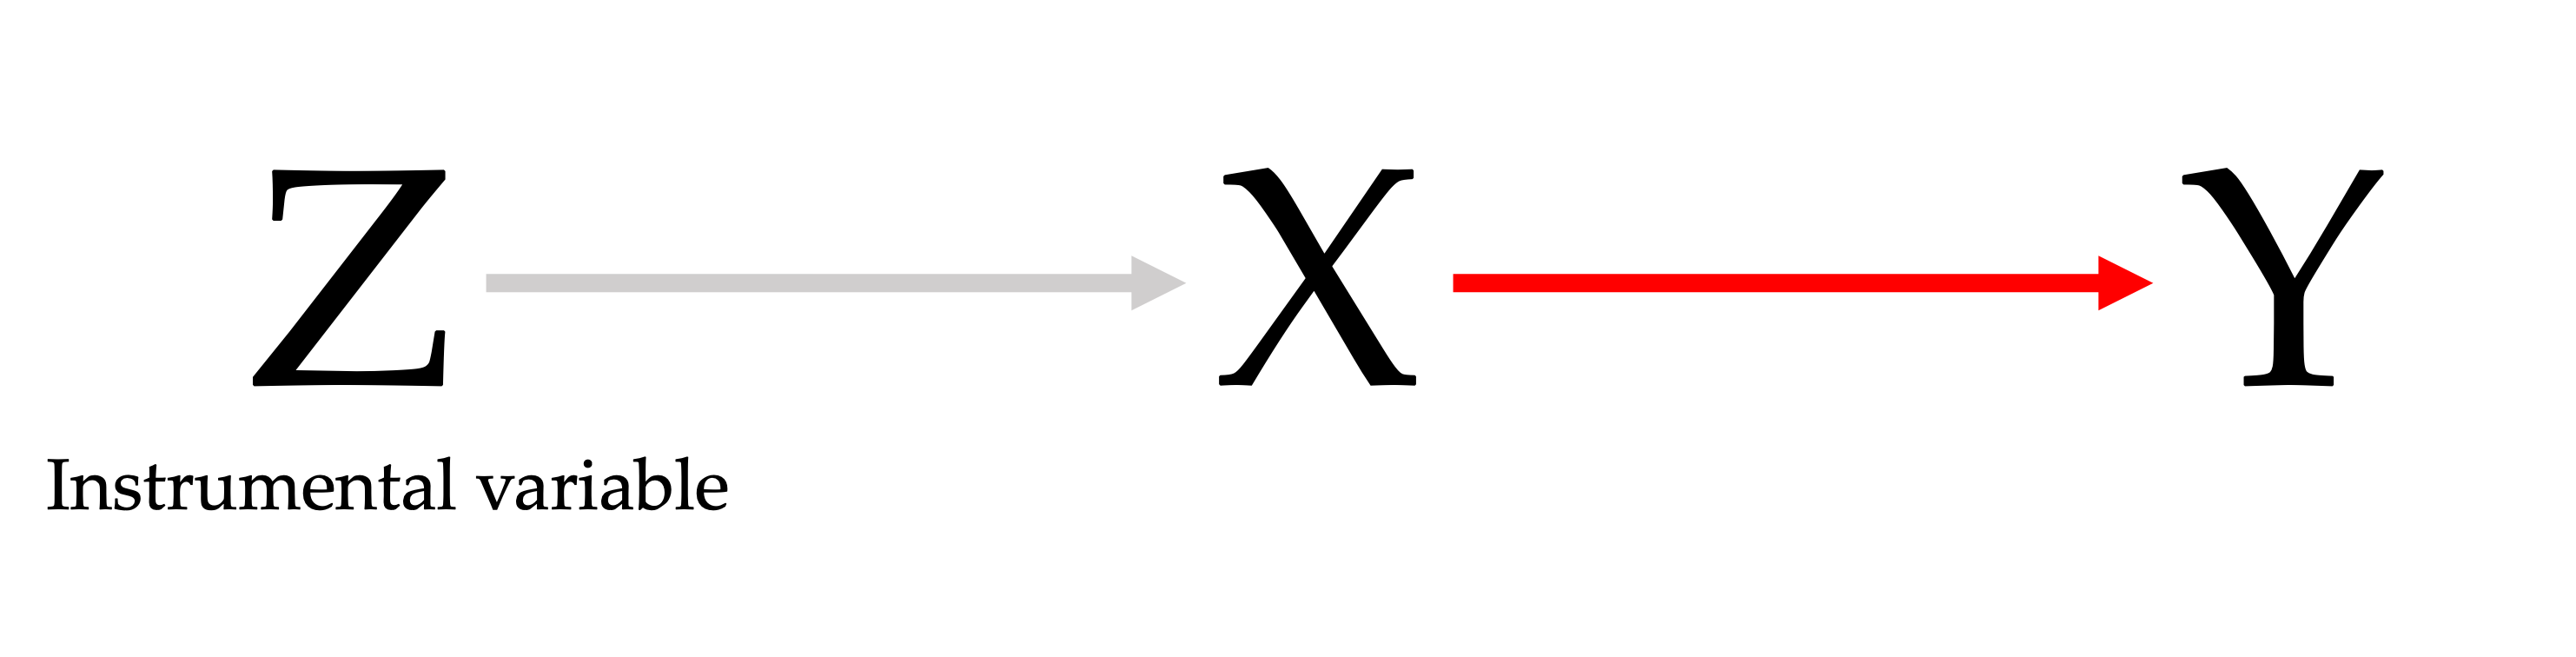
\includegraphics[width=\textwidth]{DAGs/iv_relevance.png}
\end{figure}

\end{frame}


\begin{frame}{Does IV always work?}

\begin{itemize}
    \item No! It only works if we have a valid instrument
    \item For this, we need three conditions:
\end{itemize}

2. Independence/Exogeneity: $Z$ is as good as randomly assigned

\begin{figure}
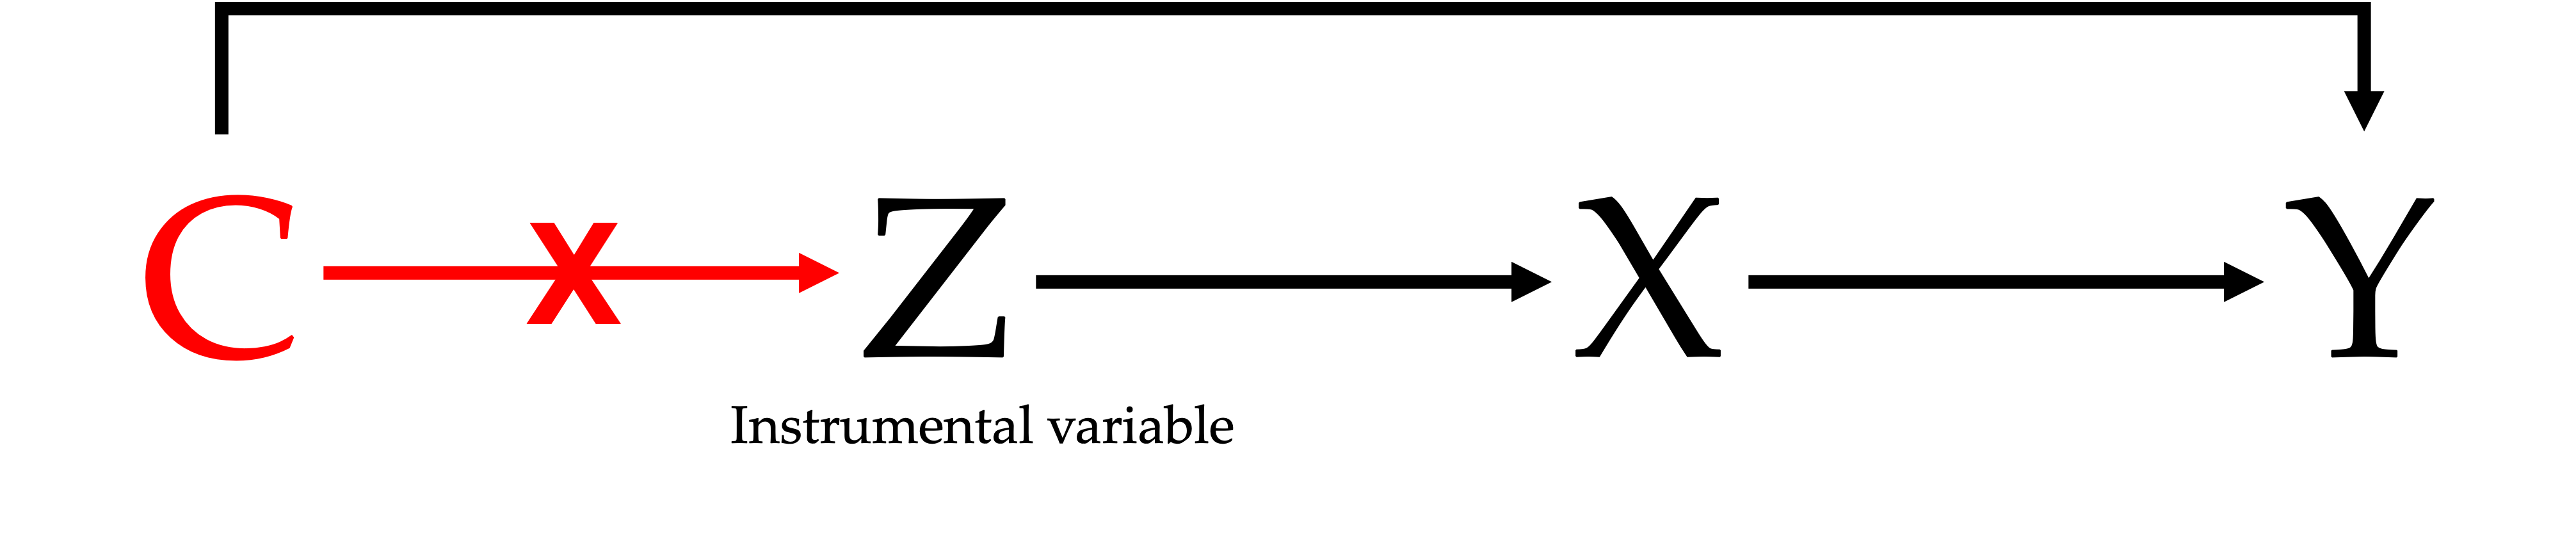
\includegraphics[width=\textwidth]{DAGs/iv_independence.png}
\end{figure}

\end{frame}



\begin{frame}{Does IV always work?}

\begin{itemize}
    \item No! It only works if we have a valid instrument
    \item For this, we need three conditions:
\end{itemize}

3. Exclusion: The \textbf{ONLY} way that $Z$ affects $Y$ is via $X$!
\begin{figure}
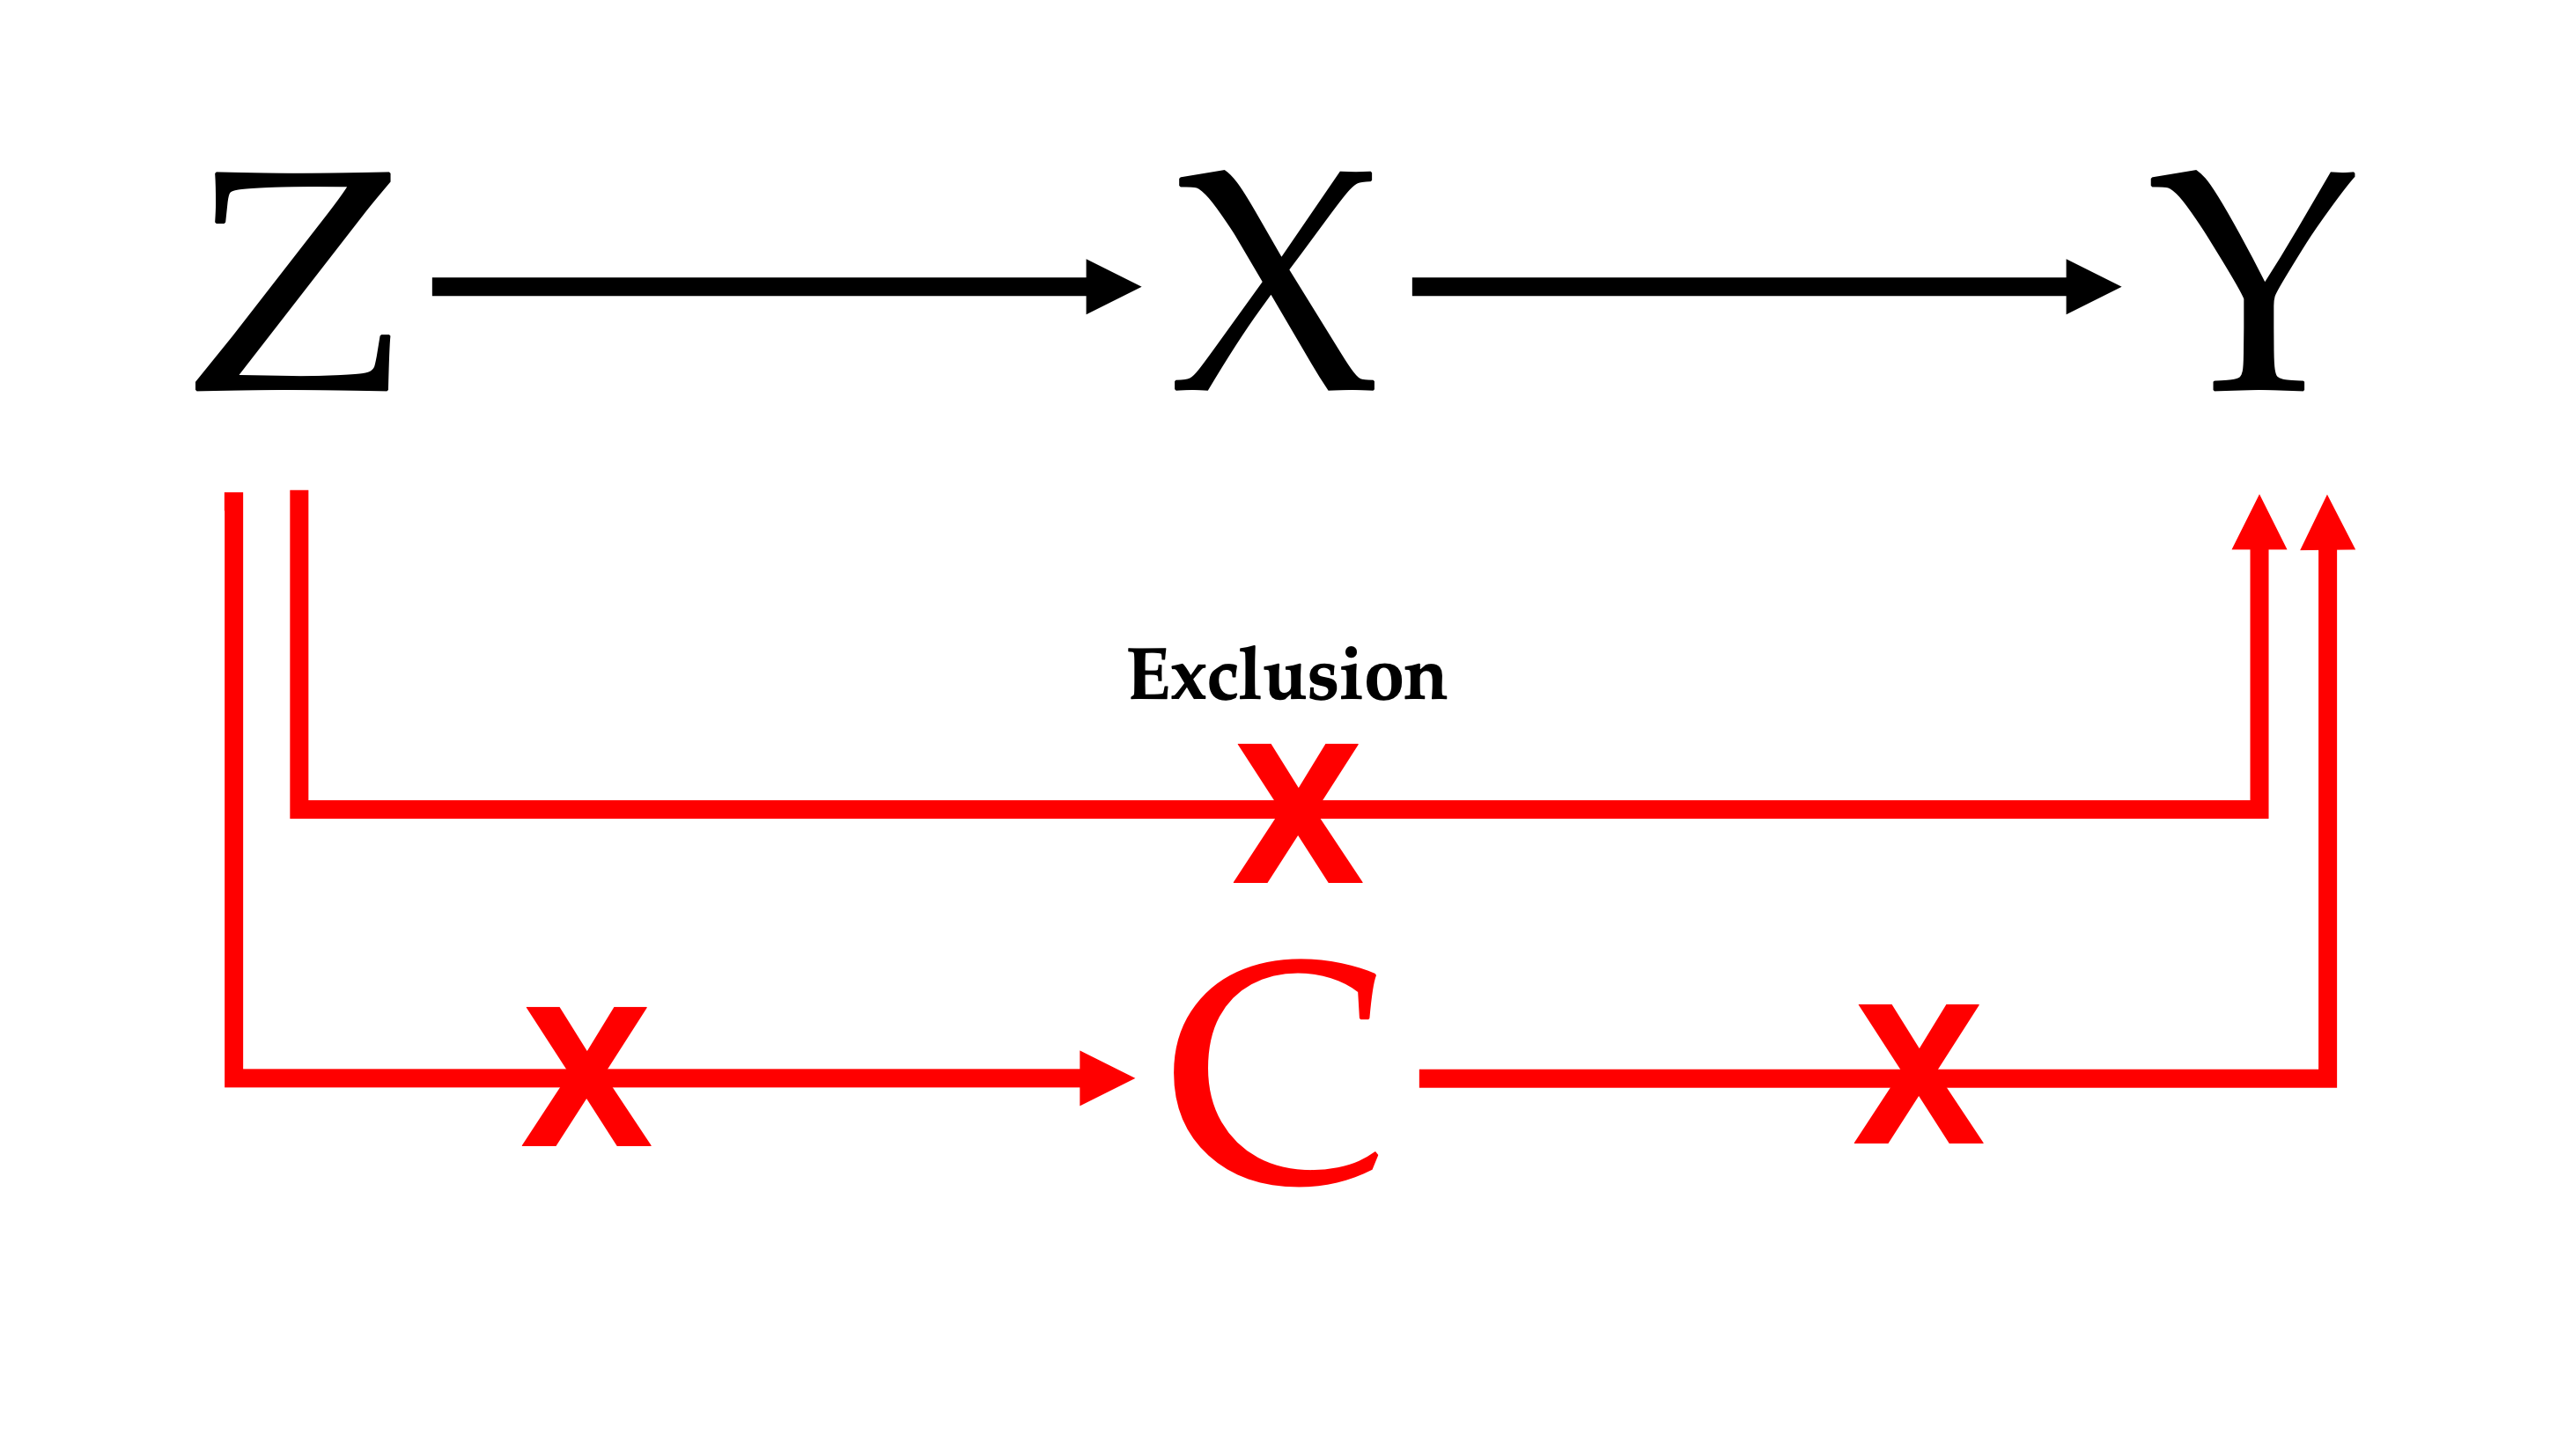
\includegraphics[width=\textwidth]{DAGs/iv_exclusion.png}
\end{figure}

\end{frame}




\section{IV Summary}



\begin{frame}{IV summary}

We need the following three assumptions for IV to work: 
    \begin{enumerate}
    \item \textbf{Relevance}: $Z$ must truly affect $X$
    \item \textbf{Independence/Exogeneity}: $Z$ is as good as randomly assigned
    \item \textbf{Exclusion Restriction}: The \textbf{only} way that $Z$ affects $Y$ is via $X$.
    \end{enumerate}



    \begin{figure}
 
        \centering
        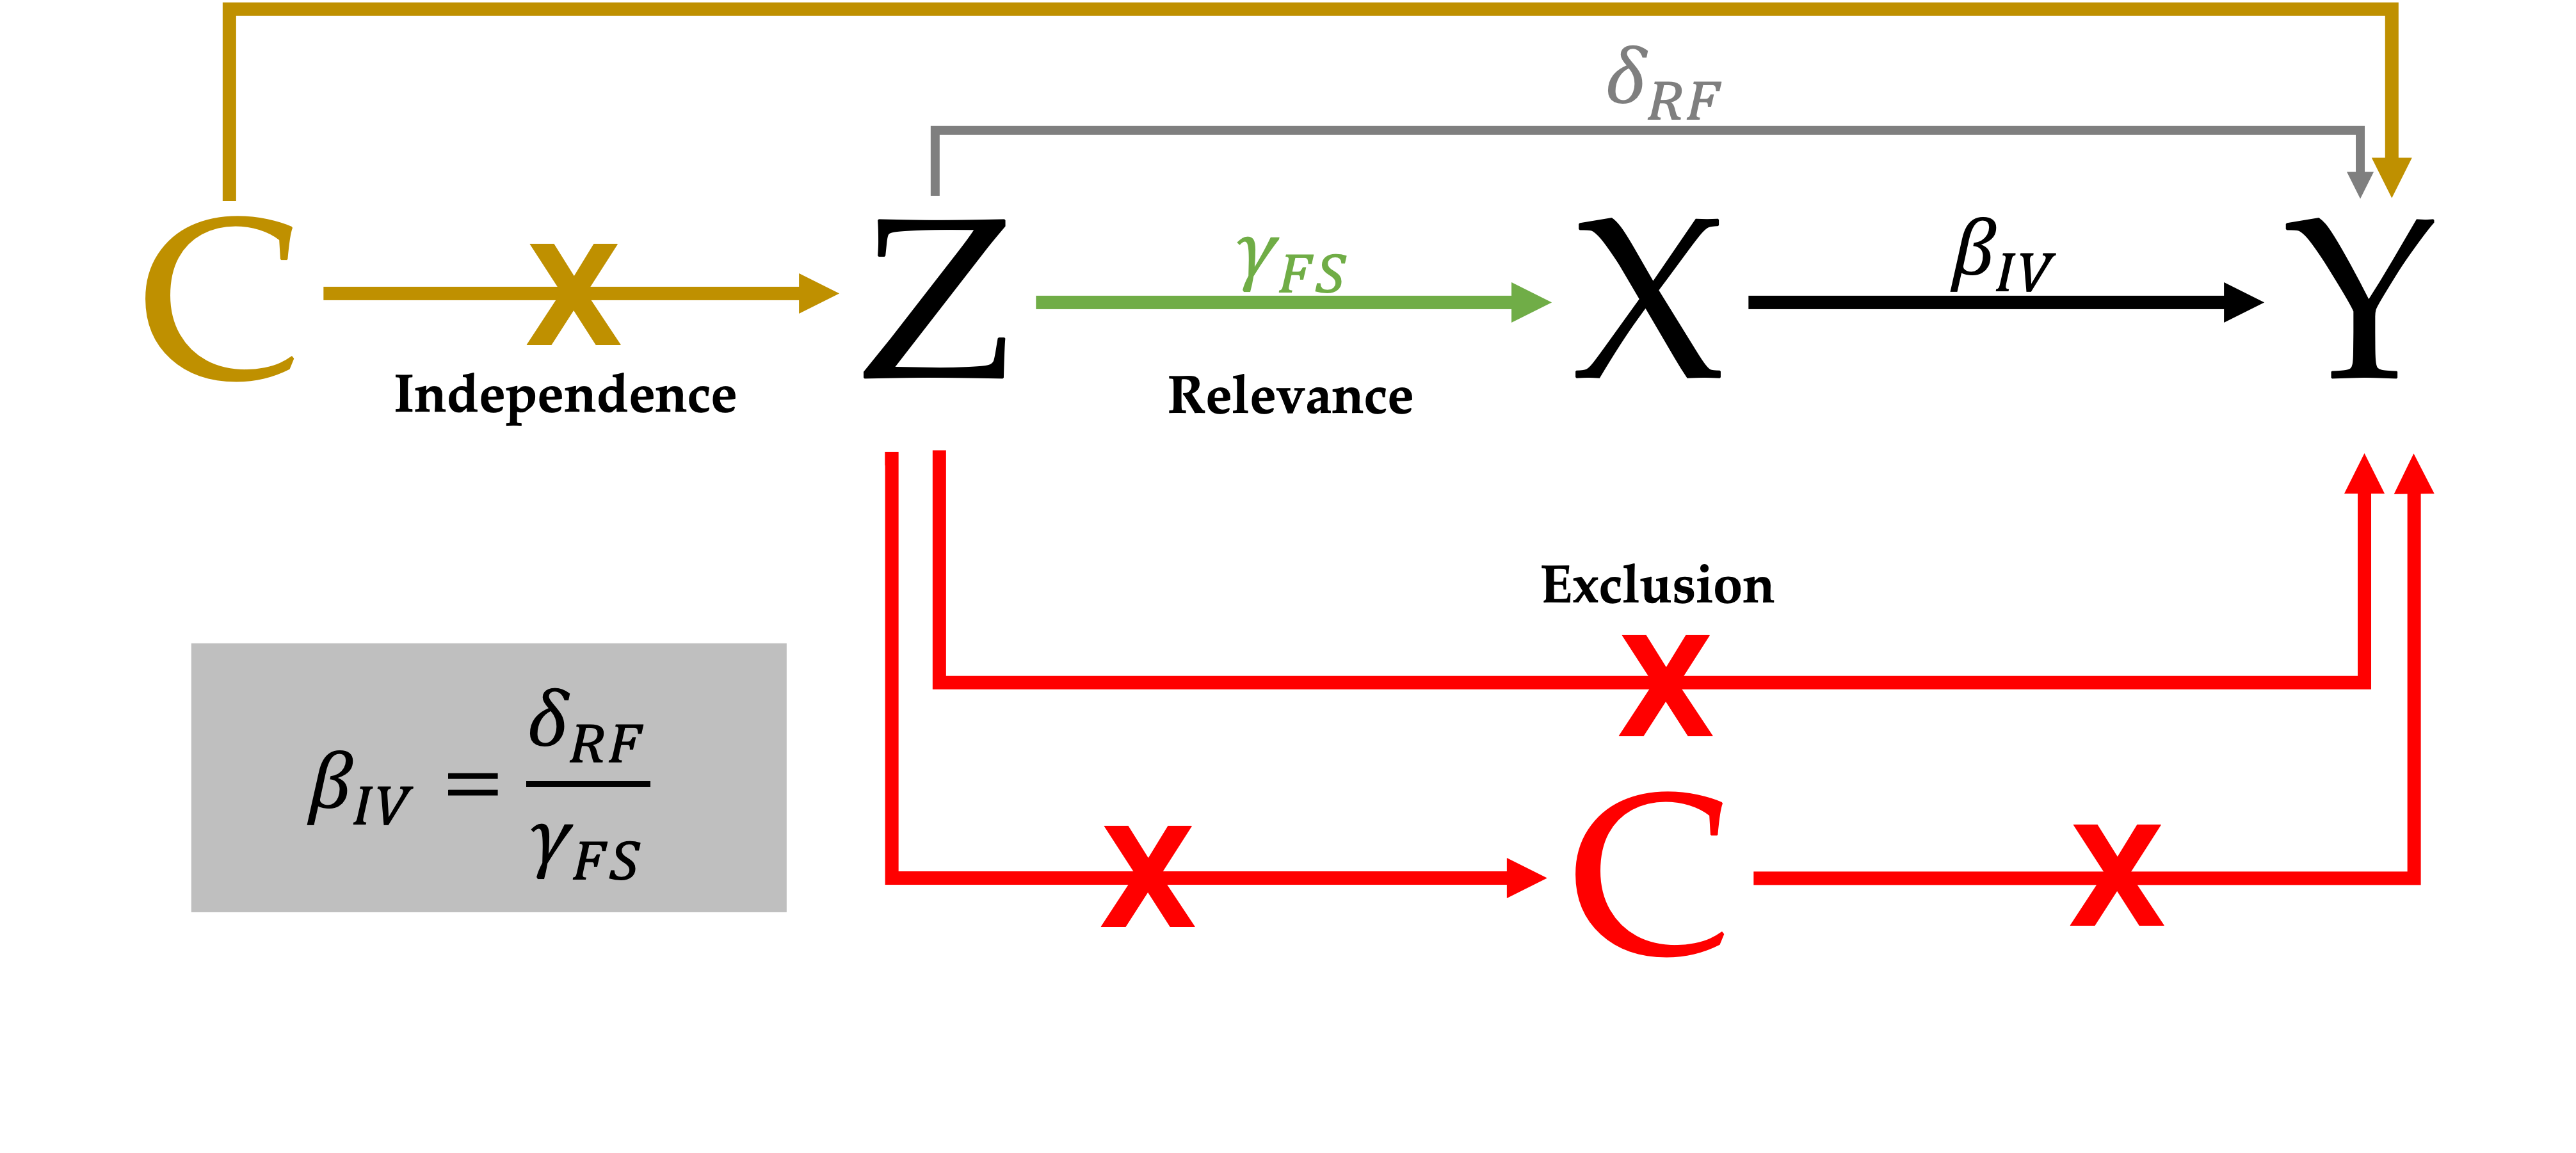
\includegraphics[width=1\textwidth]{DAGs/iv_summary_full.png}
        %\caption{Almost all you need to know about IVs!}
        \label{fig:iv3}
    \end{figure}
    
   \end{frame}



















\begin{frame}{How IV estimates can be different from OLS estimates}
    \begin{itemize}
        \item \textbf{OVB:} If OLS had omitted variable bias, and our instrument is valid, then the IV estimate should be different. We can check whether this is plausible with the OVB formula
        \item \textbf{Measurement error:} If we have random measurement error in the independent variable ($X$), then we can use IV to overcome this. In that case, the IV coefficient will be larger (in absolute value) than the OLS coefficient
        \item \textbf{LATE:} OLS gives us  ATT + Selection Bias, while IV gives us the treatment effect on the compliers (LATE). The ATT may be different from LATE, even without selection bias.
        \item \textbf{Invalid IV:} Hard to determine  what exactly is going on
        \item \textbf{Sampling variation}: This can just happen by chance
        
    \end{itemize}
    
\end{frame}












\begin{frame}{IV and controls}
    \begin{itemize}
        \item There is a catch in IV: independence (exogeneity) and exclusion restriction only need to hold \textbf{conditionally}
        \item This means: If we \textbf{know} C, we can control for it in the IV regression, and the concerns go away
        \item But then, we have the old OLS problems again (we maybe need to control for lots of things)
        \item So we should only do this in cases where we really know all the C's.    
    \end{itemize}
    
\end{frame}




\questionslide

\section{Group work}



\begin{frame}{Group work}

    \begin{itemize}
    
    
\item[\textit{Group 1:}] We are interested in the effect of being in the army on crime. We instrument being in the army with a lottery (\link{https://www.aeaweb.org/articles?id=10.1257/app.3.2.119}{paper})
%\item[\textit{Group 2:}]  We are interested in the effect of protestant religion on economic growth. We instrument protestantism in a region with the distance to Wittenberg (\link{https://academic.oup.com/qje/article/124/2/531/1905076}{paper})

\item[\textit{Group 2:}]  We are interested in the effect of income on conflict. We instrument income with rainfall (\link{https://www-journals-uchicago-edu.libproxy.berkeley.edu/doi/10.1086/421174}{paper})


\item[\textit{Group 3:}]  We are interested in the effect of air pollution on mortality. We instrument local air pollution with wind direction (\link{https://www.aeaweb.org/articles?id=10.1257/aer.20180279}{paper})



       \end{itemize}

\begin{enumerate}
	\item Relevance: Z must truly affect X
	\item Independence/Exogeneity: Z is as good as randomly assigned
	\item Exclusion restriction: The \textbf{only} way that Z affects Y is via X
\end{enumerate}

%\textbf{\alert{Your job: Discuss whether these three assumptions hold!!}}

 %  \begin{alertblock} {\centering \vspace{-1.5ex} \\ Your job: Discuss whether these three assumptions hold!  \\ \vspace{-1.5ex} } \end{alertblock}
    
    \task{Your job: Discuss whether these assumptions hold!}
   \end{frame}







\questionslide




\end{document}
